% vim: spell spelllang=en_gb
\chapter{Methods}

This section discusses and motivates the methods used in the project. Figure \ref{fig:flow_chart}
shows a flow chart of the pipeline (an enlarged copy is available in Figure \ref{fig:flow_chart_big}
of Appendix \ref{appendix:raw}). The pipeline consists of the following steps: Data collection, text
classification, location extraction, and visualization. Python is the primary programming language
used for the project because of the rich ecosystem surrounding it, especially when it comes to data
science-related tasks. The code base is available at a GitHub
repository\footnote{https://github.com/YasserKa/Classification-and-visualization-of-natural-disasters-using-Twitter}
accompanied with a \texttt{README.md} containing instructions to set up the environment and run the
project.
\begin{figure}[H]
\begin{center}
  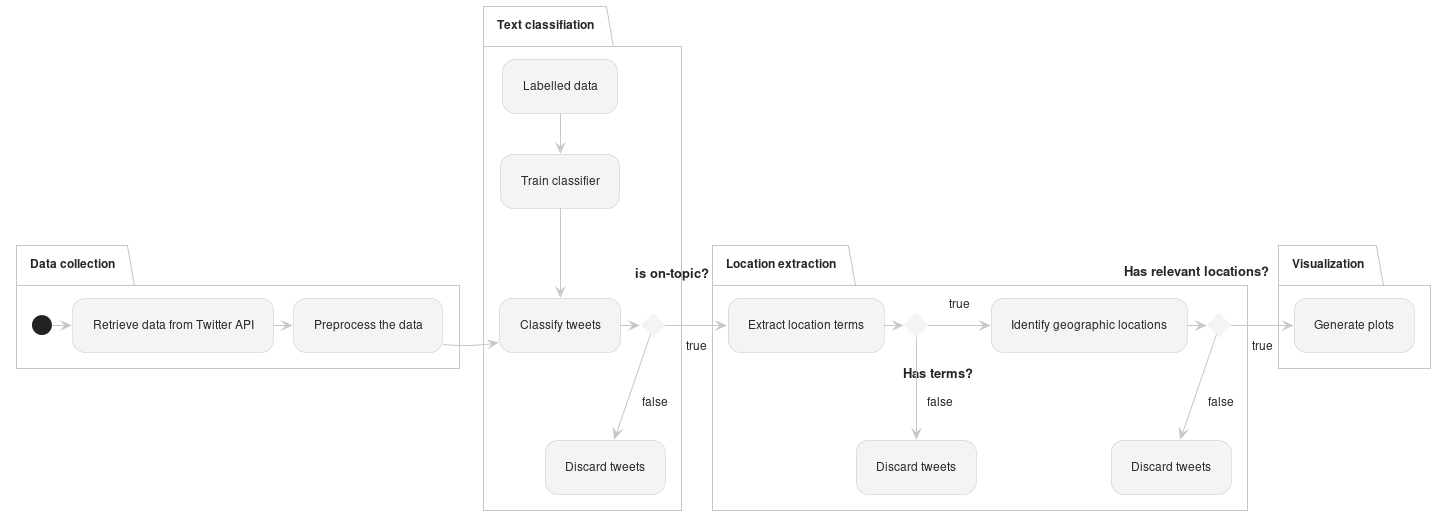
\includegraphics[width=\columnwidth]{./images/pipeline.png}
\end{center}
\caption{Flow chart for the pipeline}
\label{fig:flow_chart}
\end{figure}

\section{Data Collection}

Finding a good quality data source is the first step to having a lean start for most research
questions. The pipeline trains an \ac{ML} classifier using a manually labelled dataset containing
4899 tweets with attributes presented in Table~\ref{tab:dataset_attr}. The text and metadata of the tweets are extracted
from Twitter's API using the IDs. The trained model performance is verified using the tweets from
the API using Tweepy\footnote{https://docs.tweepy.org/en/latest/index.html}, a python library for
accessing Twitter API.

\begin{table}
  \center
  \label{tab:dataset_attr}
  \begin{tabular}{|l|l|l|}
    \hline
    Field & Type & Description \\
    \hline
    ID & Int & ID of the tweet\\
    \hline
    On Topic  & Bool & Text discusses an event \\
    \hline
    Informative sarcastic  & Bool & Text contains relevant information about the event \\
    \hline
    Contains IMPACT info & Bool & Text discusses the impact of the event \\
    \hline
    Explicit location & Bool & Text mentions the location of the event \\
    \hline
  \end{tabular}
  \caption{Dataset attributes}
\end{table}

Textual data requires pre-processing for several tasks, such as training an \ac{ML} algorithm, text
analysis, and visualization. Parts of text that don't contribute to the context are removed:
\ac{URL}s, emojis, mentions, hashtag signs, numbers, new lines, punctuation, and stopwords (provided
by spaCy\footnote{https://spacy.io/}, an \ac{NLP} python library). Afterwards, duplicate tweets,
tweets containing no text, and retweets are discarded from the dataset.

Data needs to be stored and managed to accommodate policies and regulations. Twitter's developer
policy\footnote{https://developer.twitter.com/en/developer-terms/policy} has a content
redistribution section stating that only the IDs of the tweets can be shared online. Thus, the
tweets can't be available publicly on such as GitHub, the service that hosts the publicly available
code base. To this end, the data is stored and cached after each step on google drive using
\ac{DVC}'s\footnote{https://dvc.org/doc} data management capabilities.


Twitter's API provides an extensive list of information about the
tweets\footnote{https://developer.twitter.com/en/docs/twitter-api/data-dictionary/object-model/tweet}.
It shares the engagement metrics of the tweet, including like count, reply count, and retweet count;
as well as, an \ac{NLP} analysis of its own, such as the language used, and entities parsed from the
text. Table~\ref{tab:tweet_attr} shows the tweet's attributes used in this project for the following reasons: the id to
generate the \ac{URL} of the tweet, the text for \ac{NLP} tasks, the created date for temporal
analysis, and the author id to reduce spam.

\begin{table}
  \center
  \label{tab:tweet_attr}
  \begin{tabular}{|l|l|l|}
    \hline
    Attribute & Type & Description \\
    \hline
    id & Int & The unique identifier of the requested Tweet \\
    \hline
    text & Str & The actual UTF-8 text of the Tweet \\
    \hline
    created at & Date  & Creation time of the Tweet \\
    \hline
    author id & Str & The unique identifier of the tweet creator \\
    \hline
  \end{tabular}
  \caption{Tweet attributes used}
\end{table}

\section{Text Classification}
